\subsection{Der Eventbus}
\todo{Deadline: 25.06.}

\cite{noauthor_signals_nodate}
\citeauthor{persitzky_fehlerinjektion_2023}

\begin{figure}[!hb]
	\centering
	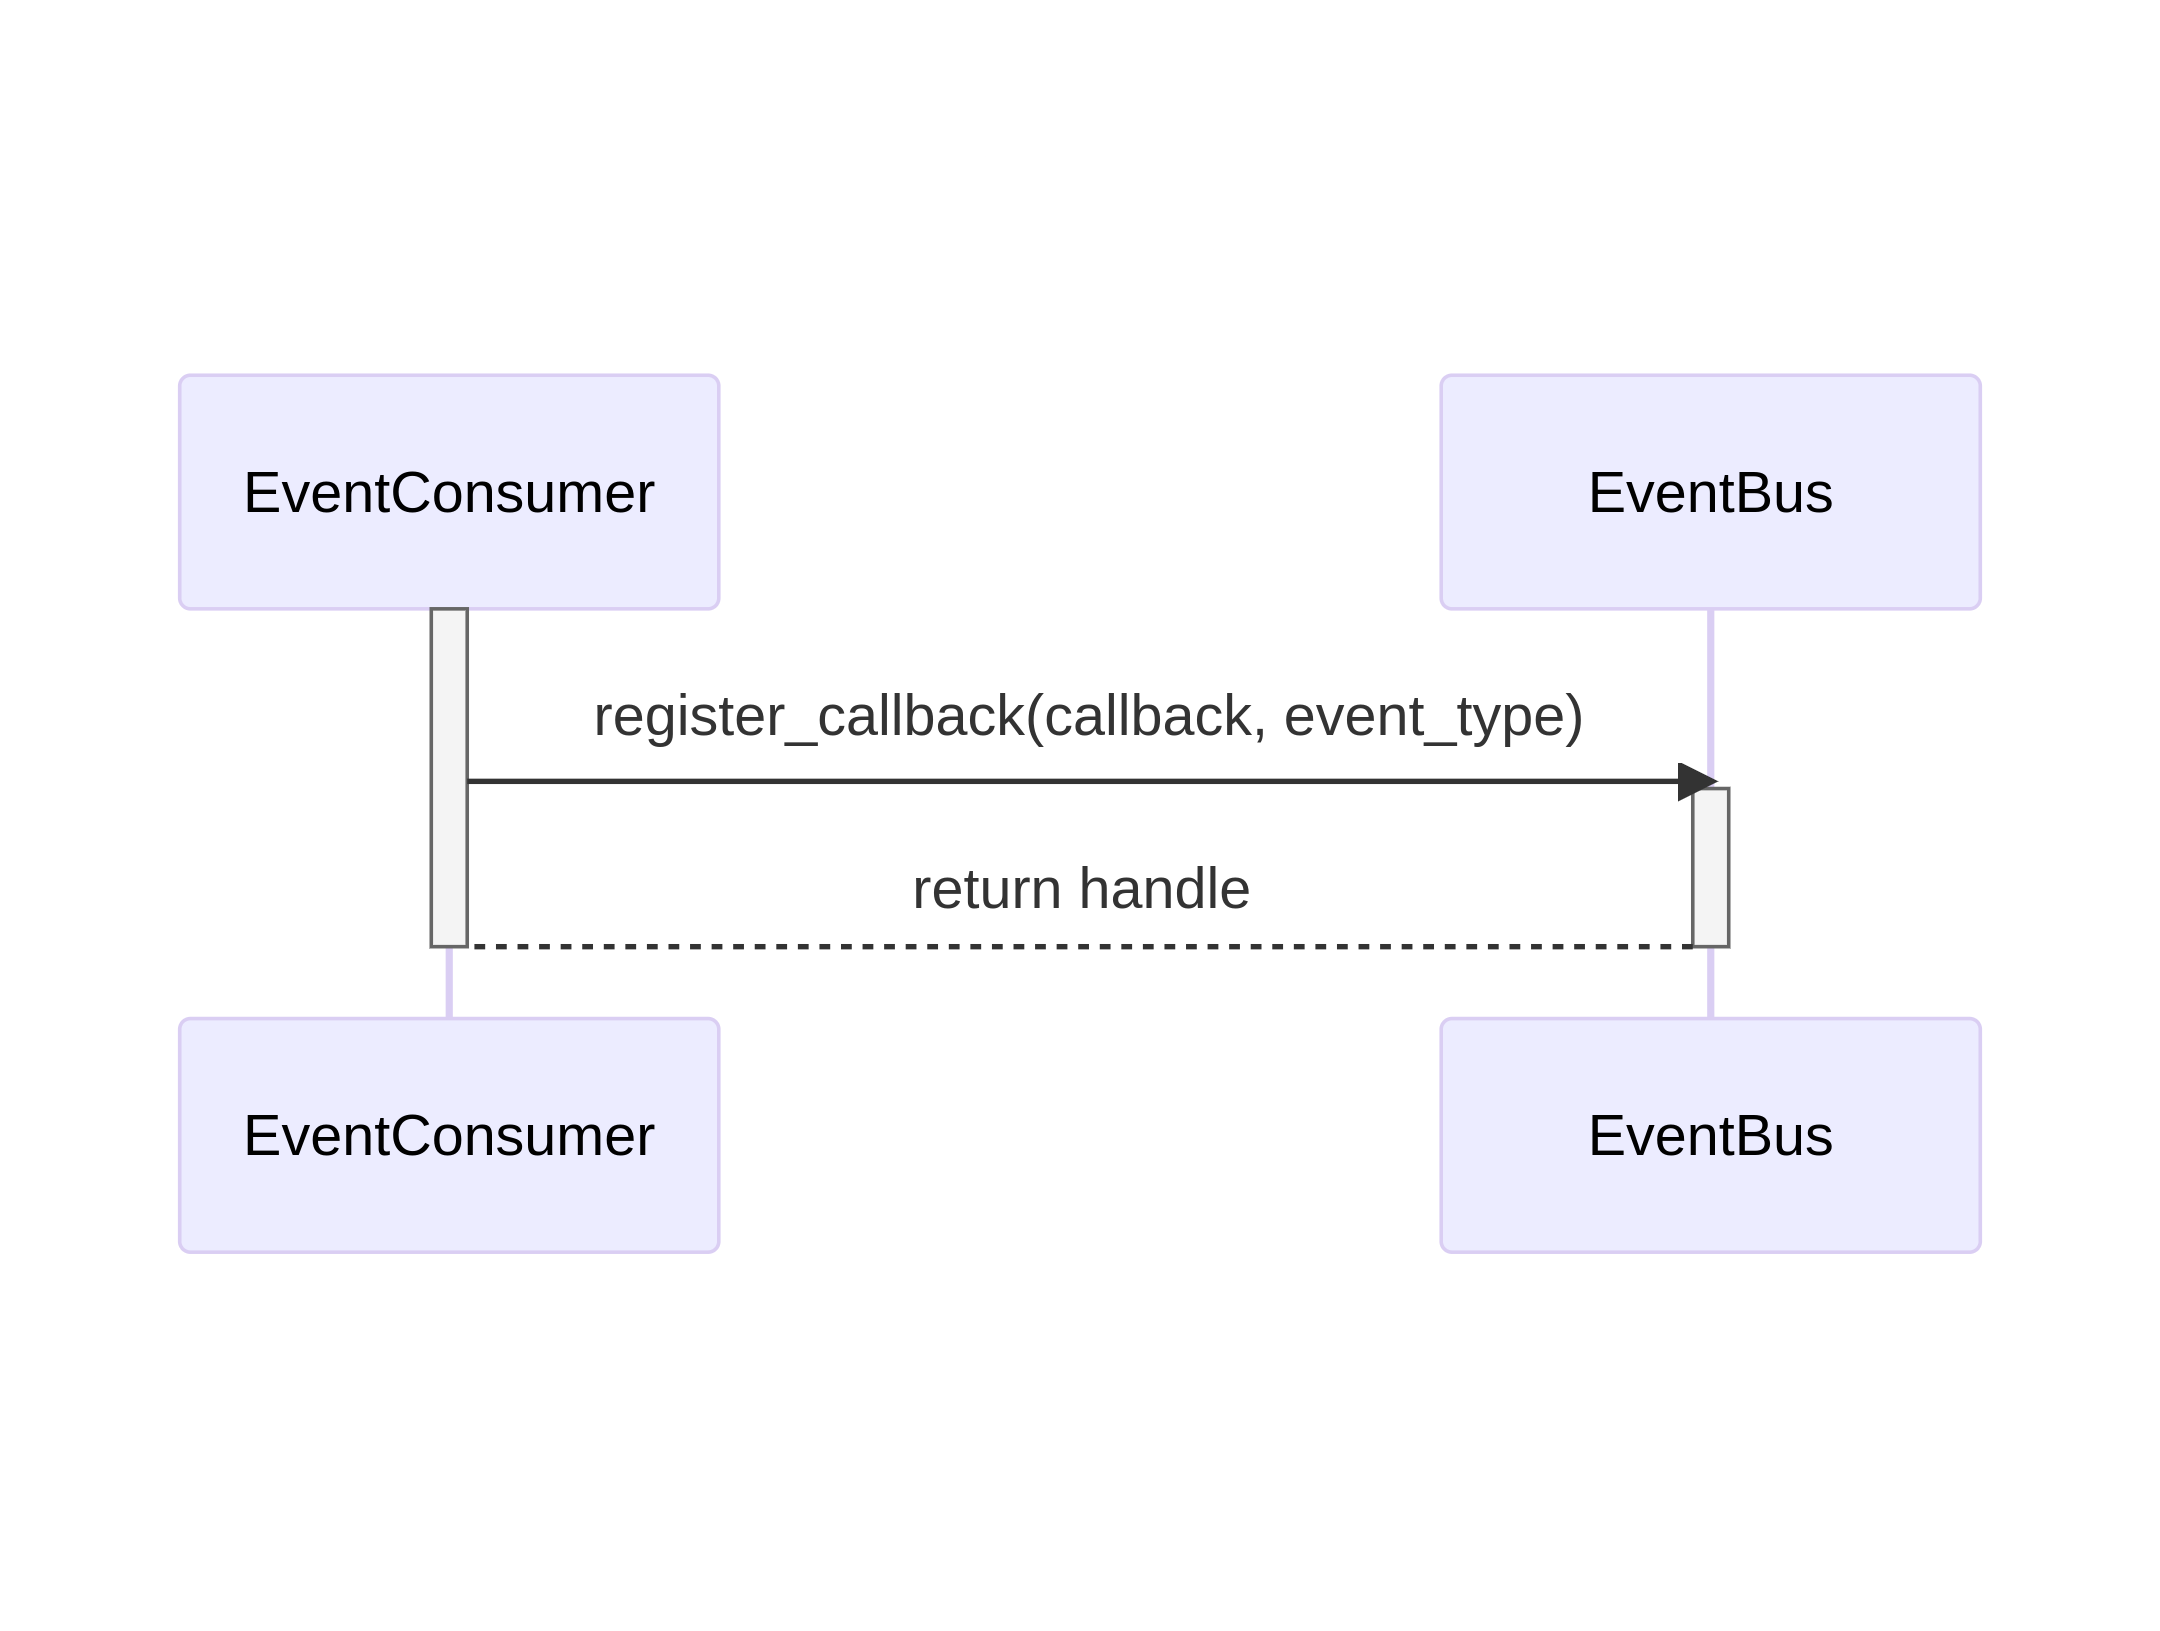
\includegraphics[width=0.75\linewidth]{images/diagrams/eventbus-register-seq.png}
	\caption{Sequenzdiagramm Registrierung Eventbus}
	\label{fig:eventbus-register-seq}
\end{figure}

\begin{figure}[!hb]
	\centering
	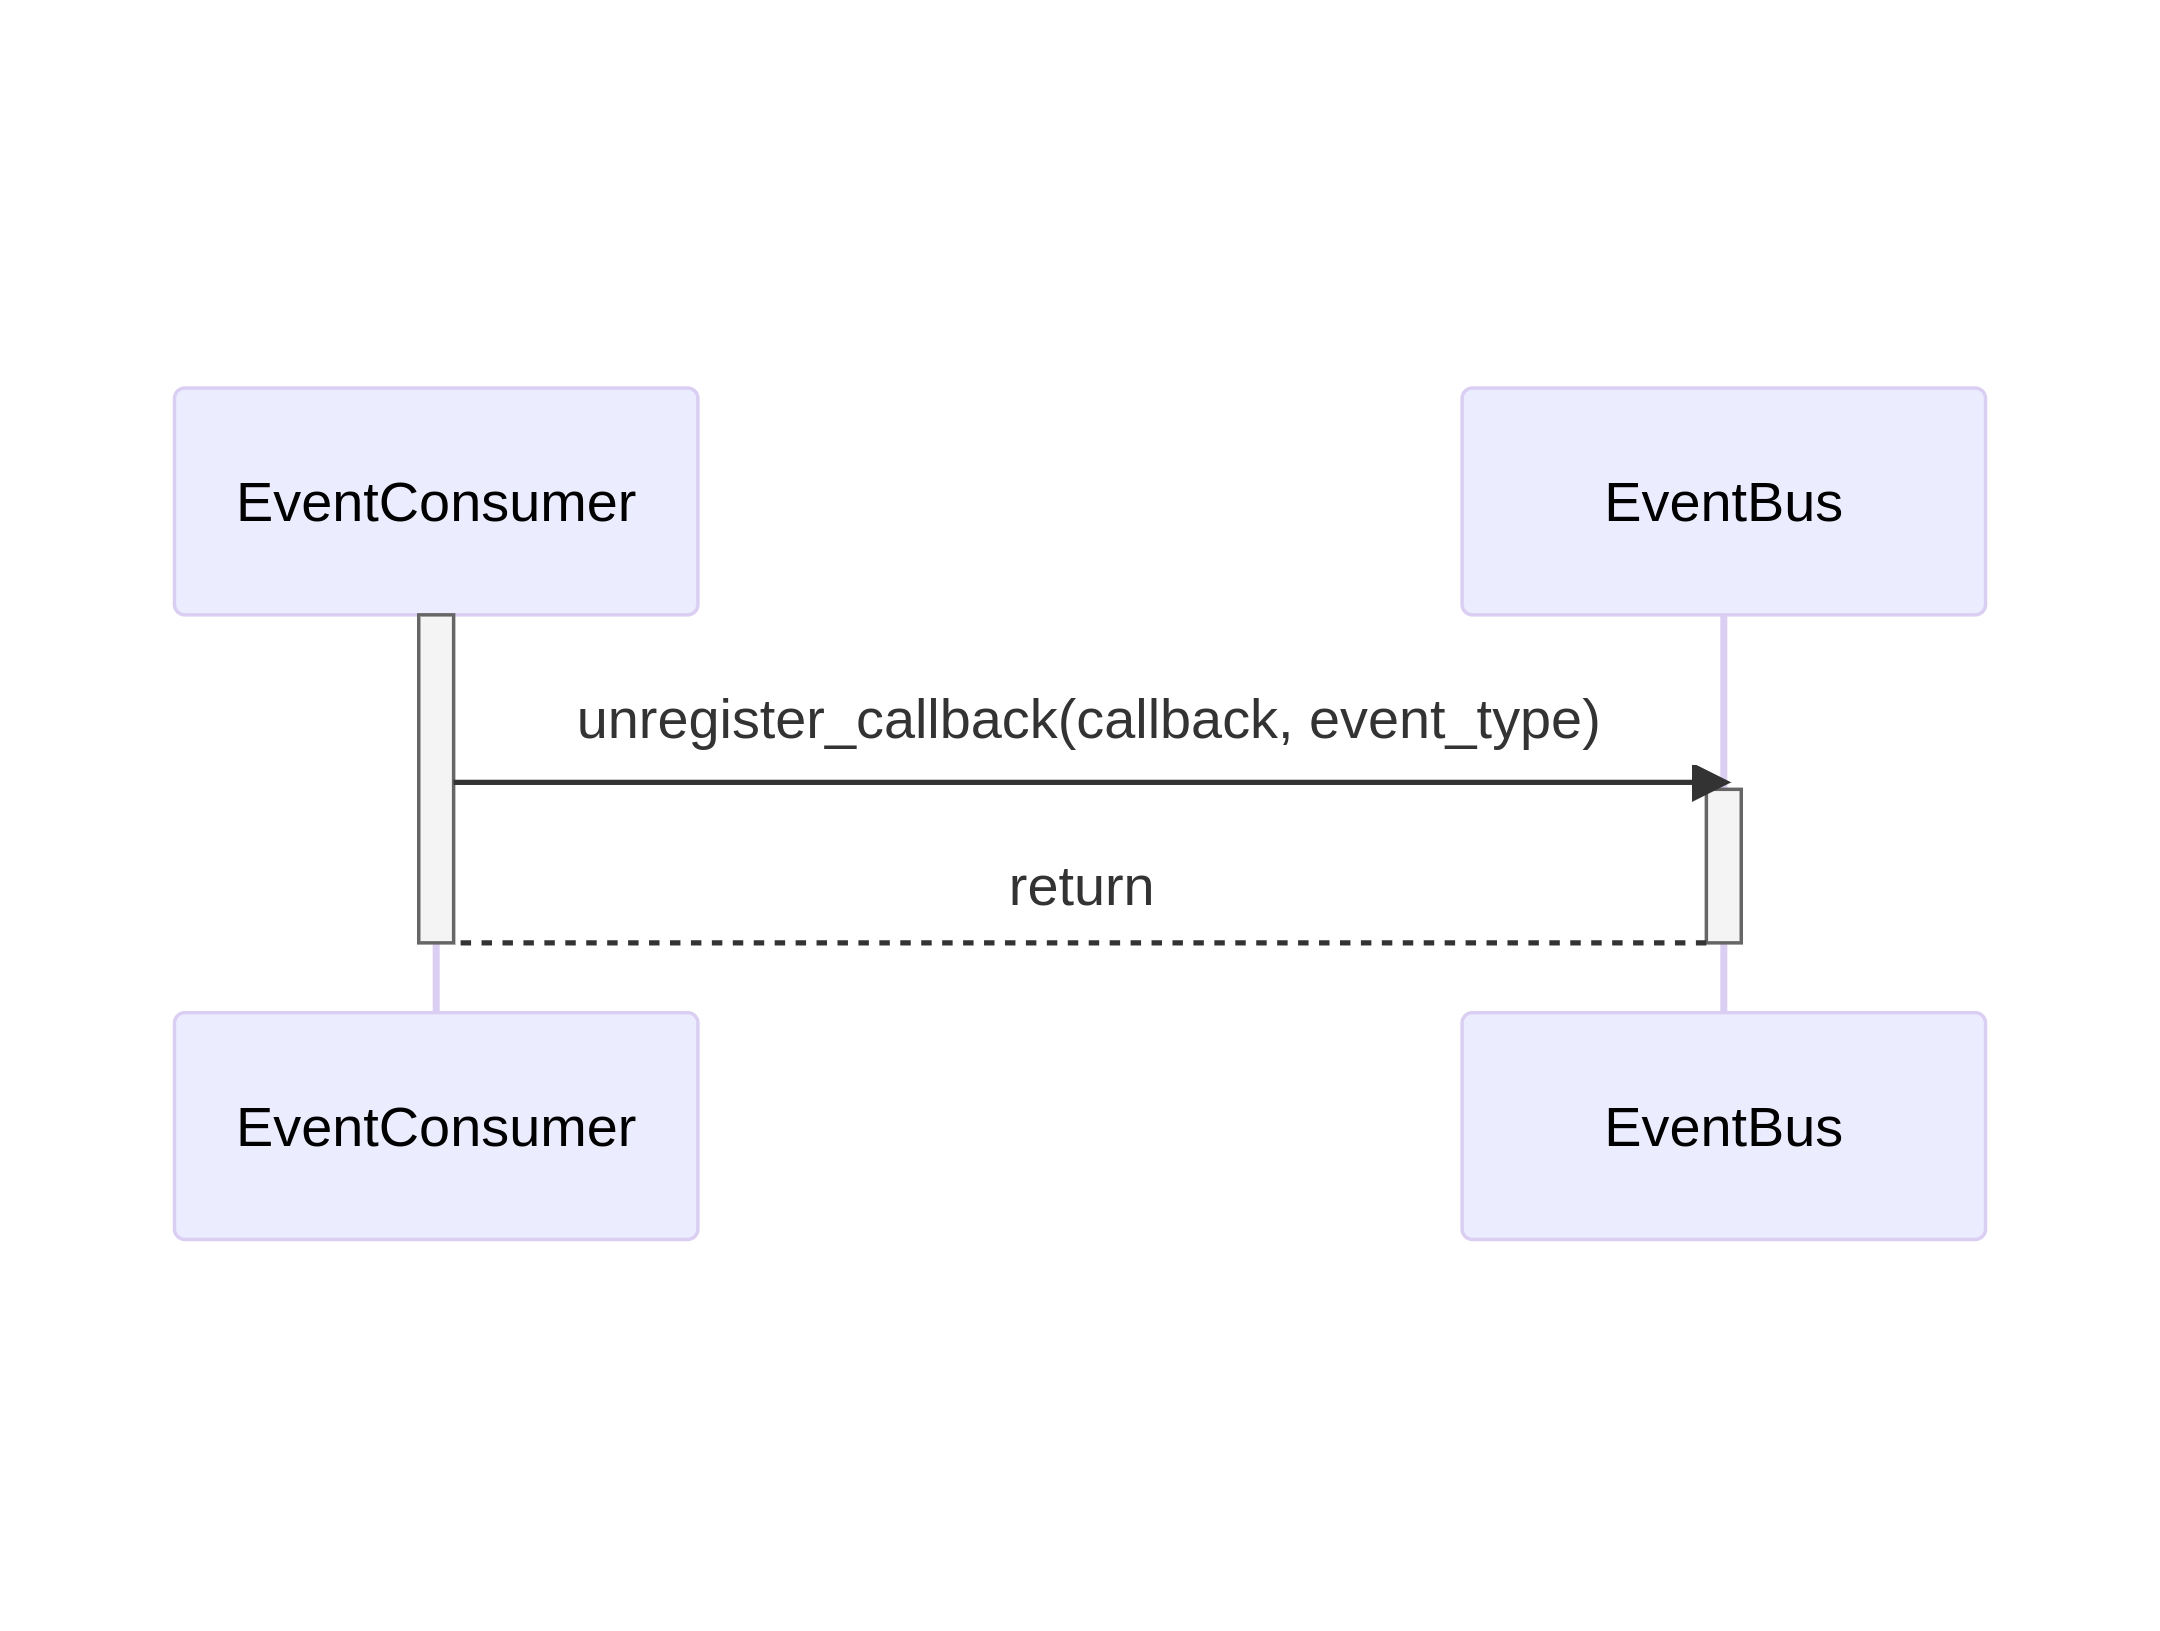
\includegraphics[width=0.75\linewidth]{images/diagrams/eventbus-unregister-seq.png}
	\caption{Sequenzdiagramm Deregistrierung Eventbus}
	\label{fig:eventbus-unregister-seq}
\end{figure}

\subsubsection*{Variante 1}

\begin{figure}[!hb]
	\centering
	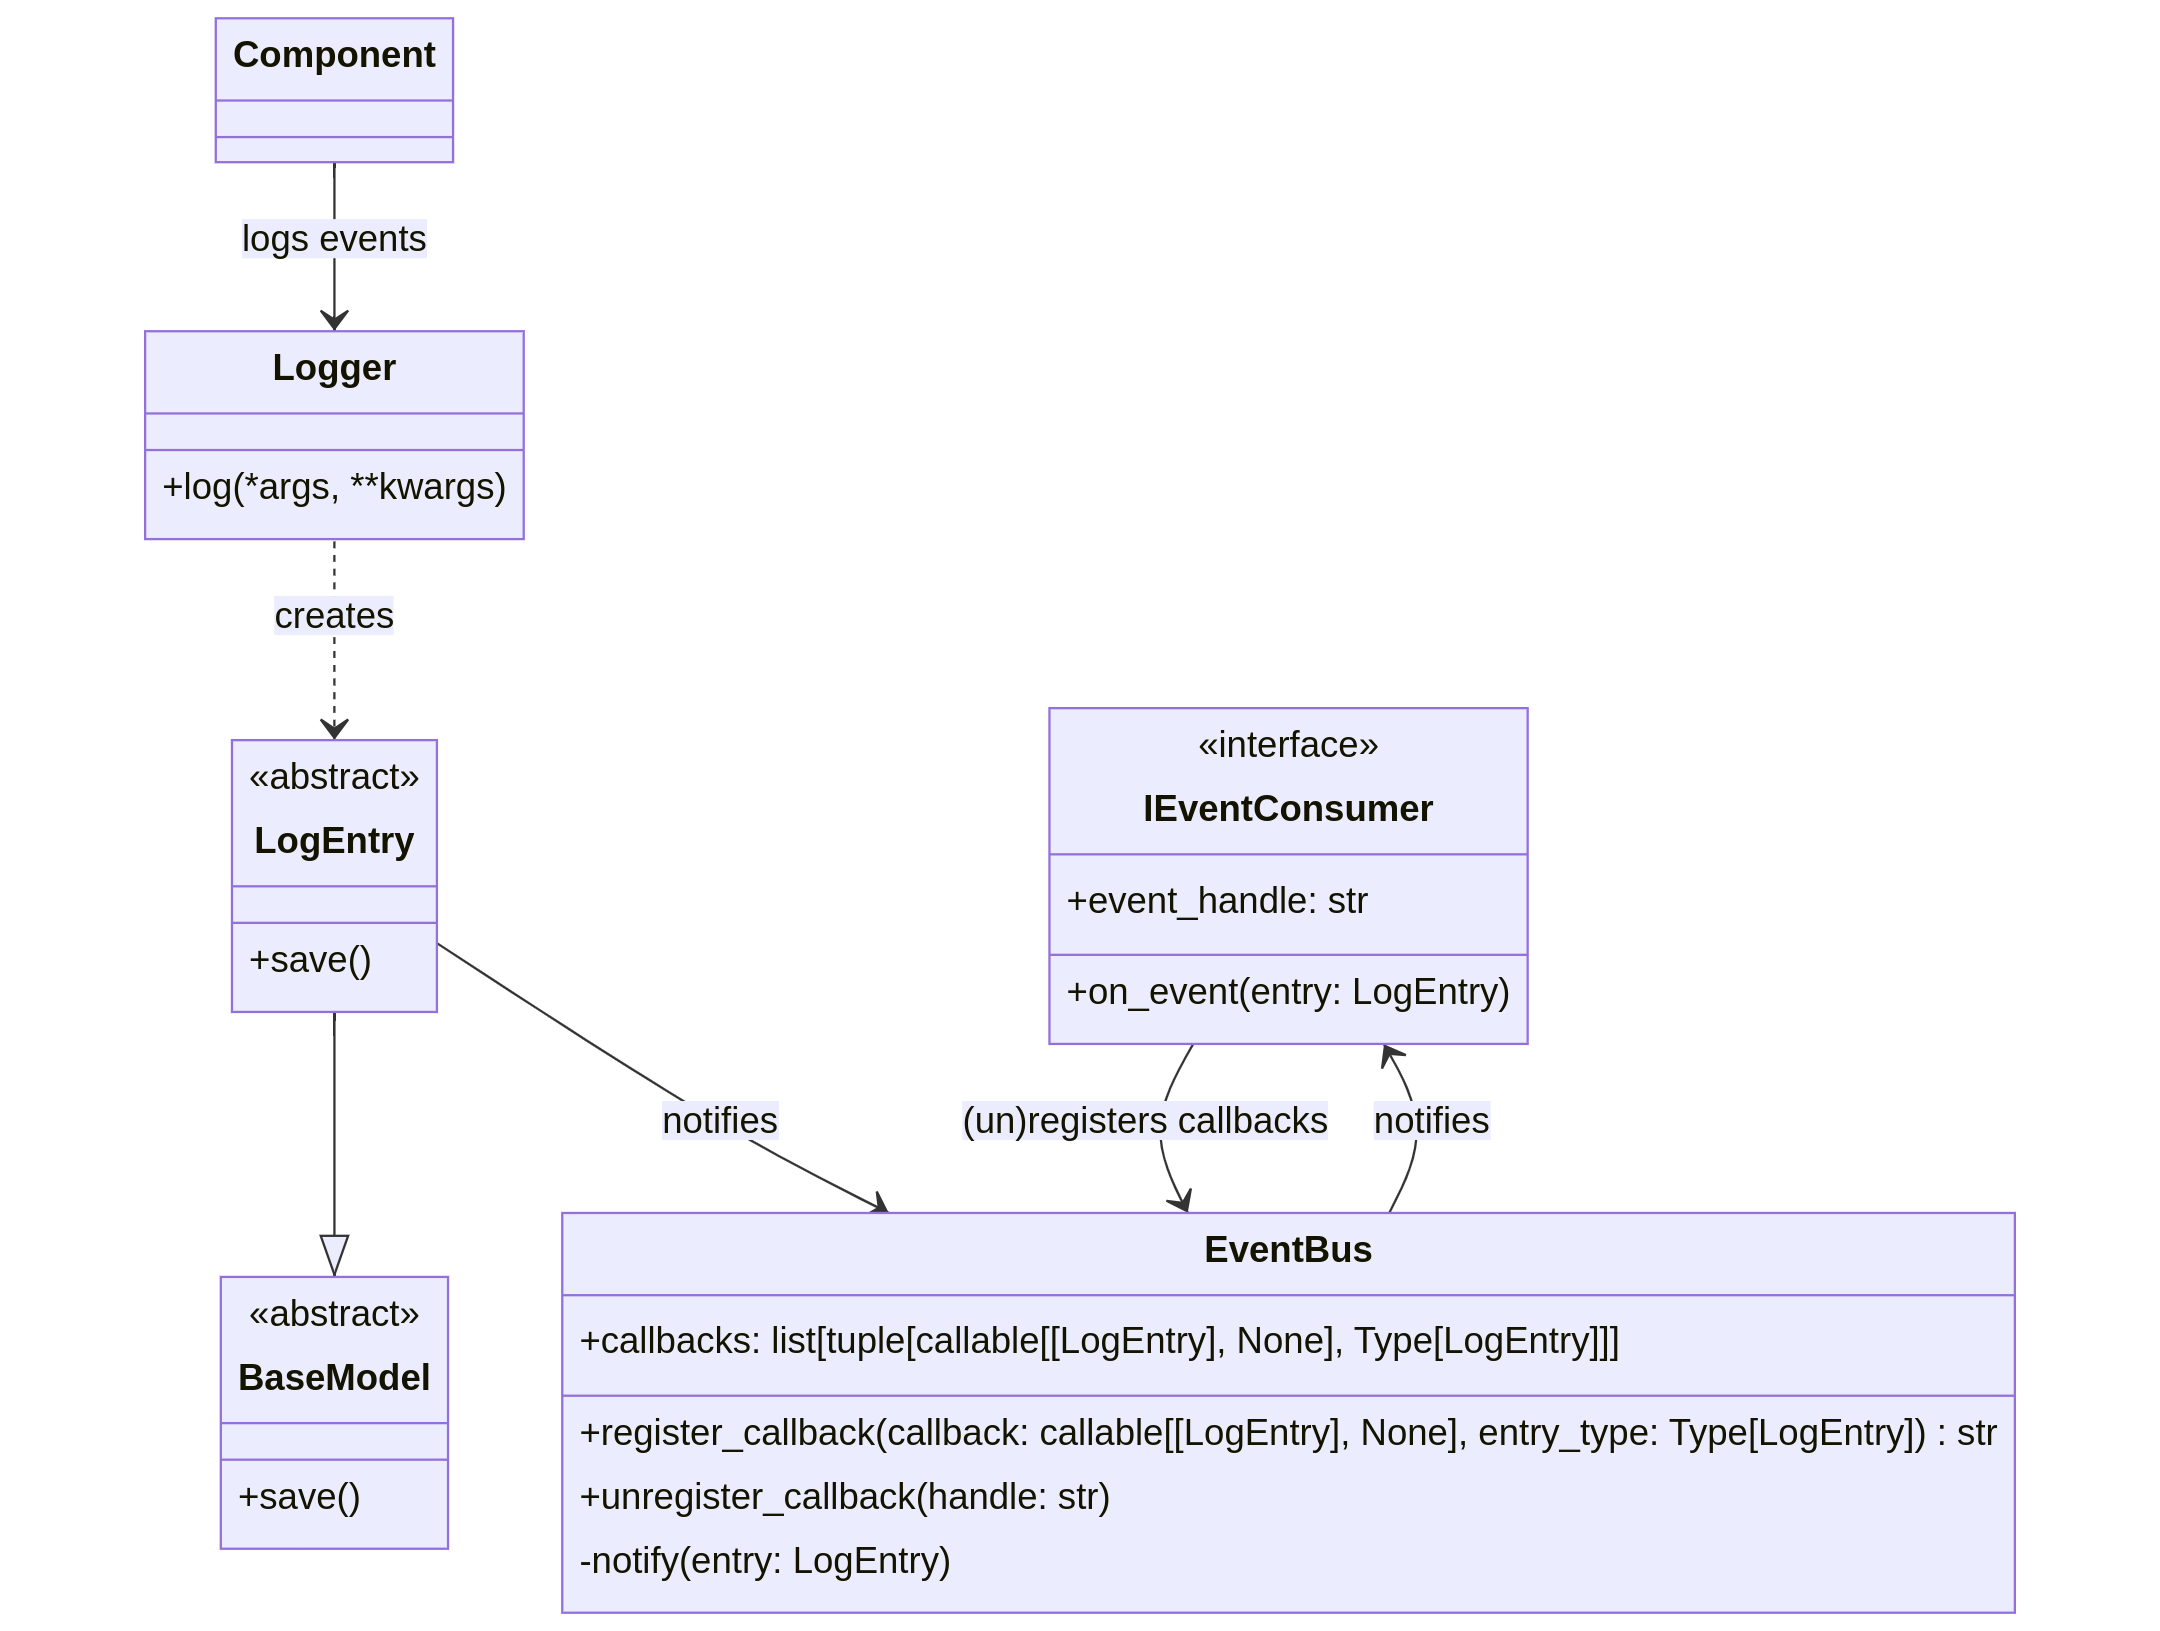
\includegraphics[width=0.75\linewidth]{images/diagrams/eventbus-v1-class.png}
	\caption{Klassendiagramm Variante 1 Eventbus}
	\label{fig:eventbus-v1-class}
\end{figure}

\begin{figure}[!hb]
	\centering
	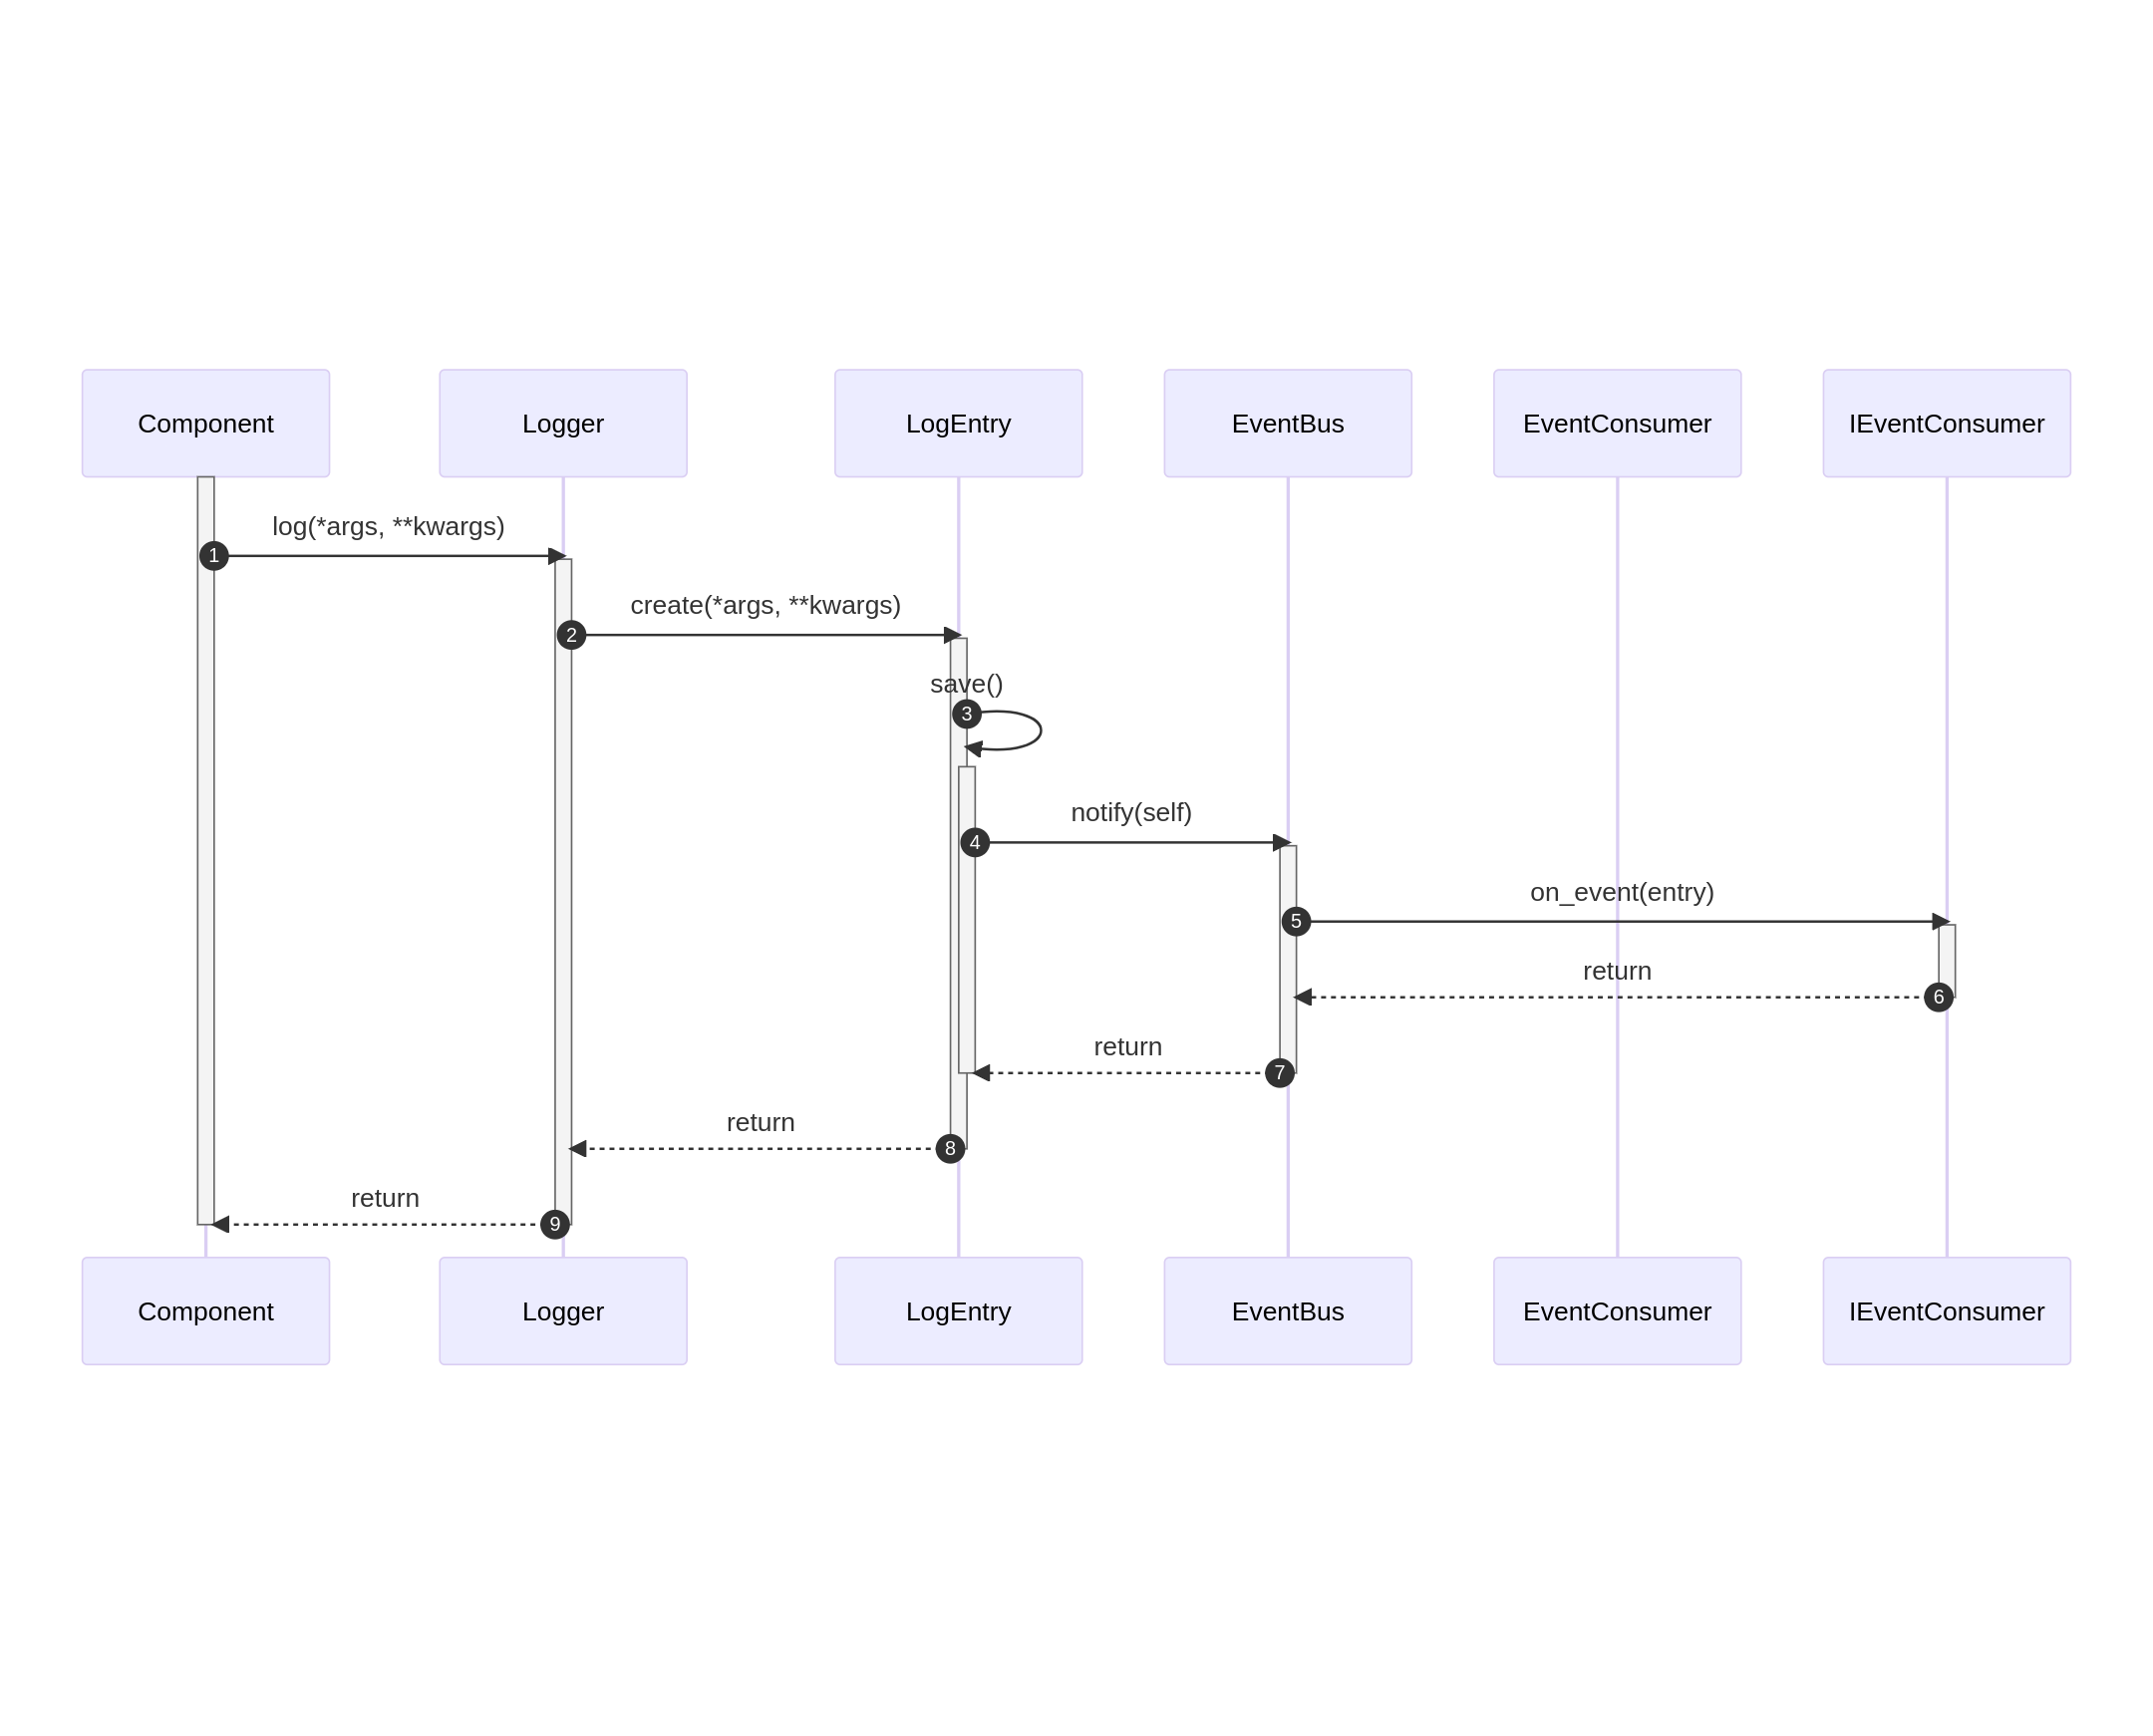
\includegraphics[width=0.75\linewidth]{images/diagrams/eventbus-v1-seq.png}
	\caption{Sequenzdiagramm Variante 1 Eventbus}
	\label{fig:eventbus-v1-seq}
\end{figure}

\subsubsection*{Variante 2}

\begin{figure}[!hb]
	\centering
	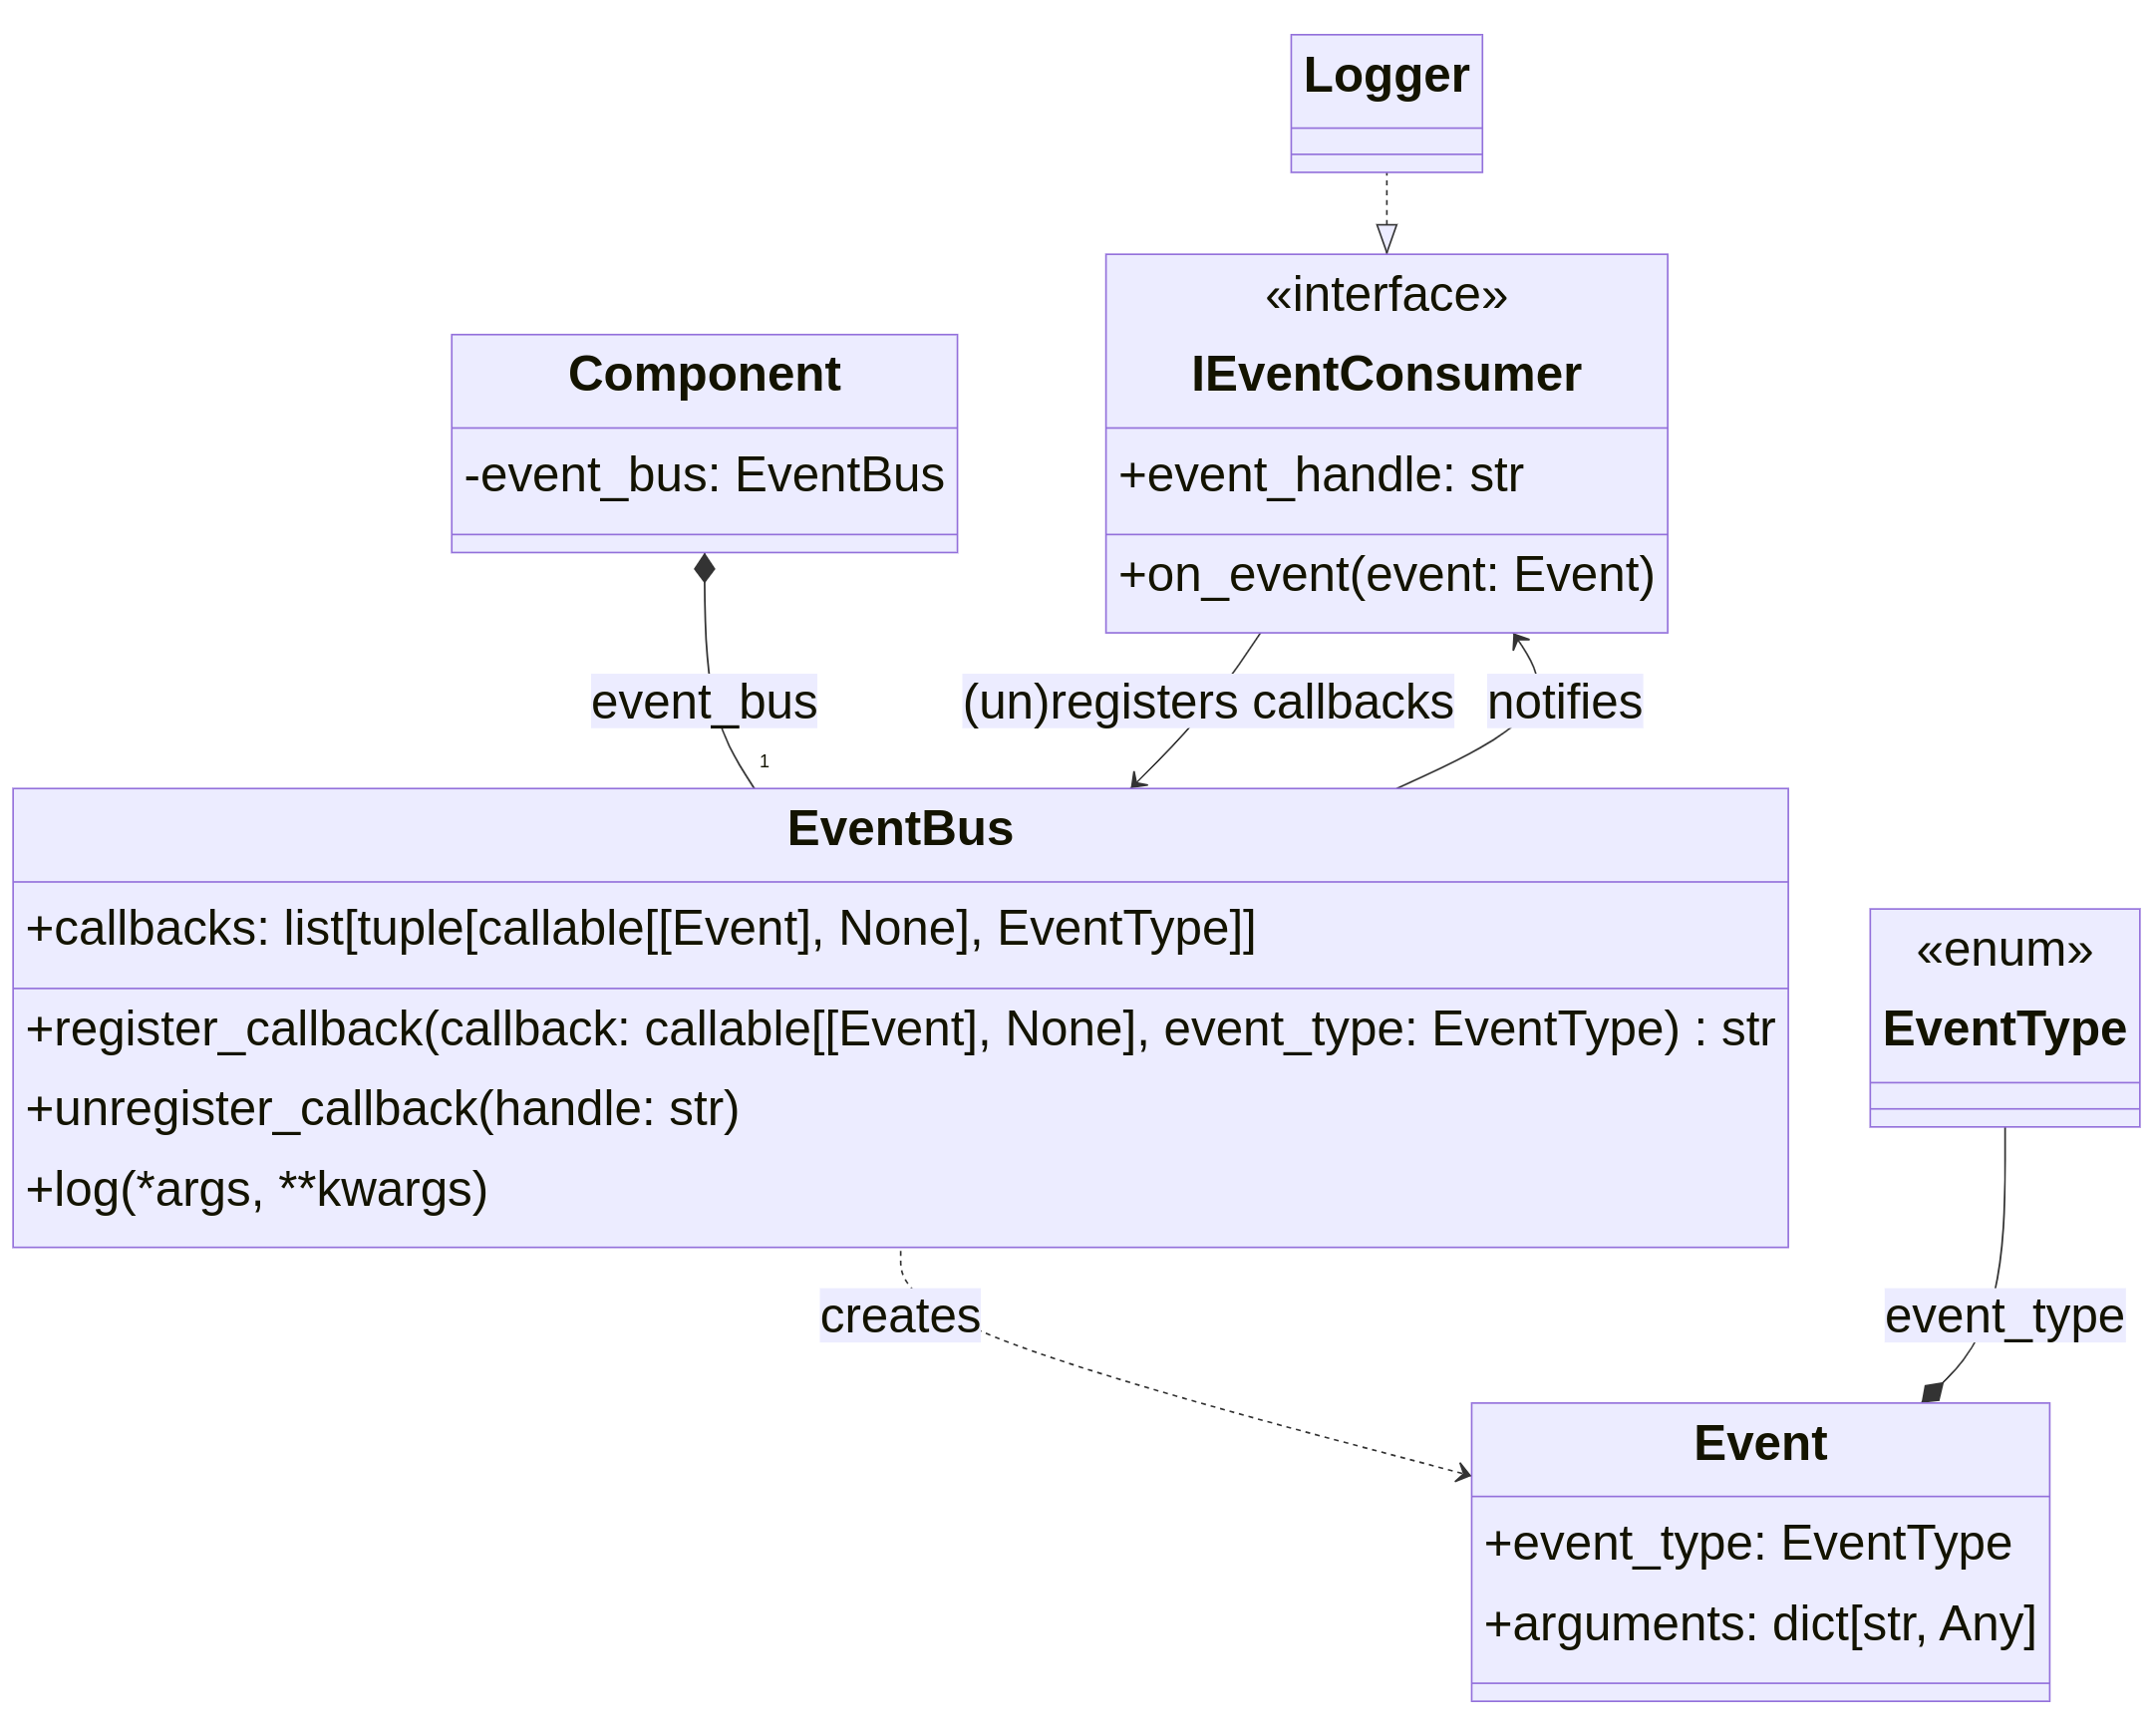
\includegraphics[width=0.75\linewidth]{images/diagrams/eventbus-v2-class.png}
	\caption{Klassendiagramm Variante 2 Eventbus}
	\label{fig:eventbus-v2-class}
\end{figure}

\begin{figure}[!hb]
	\centering
	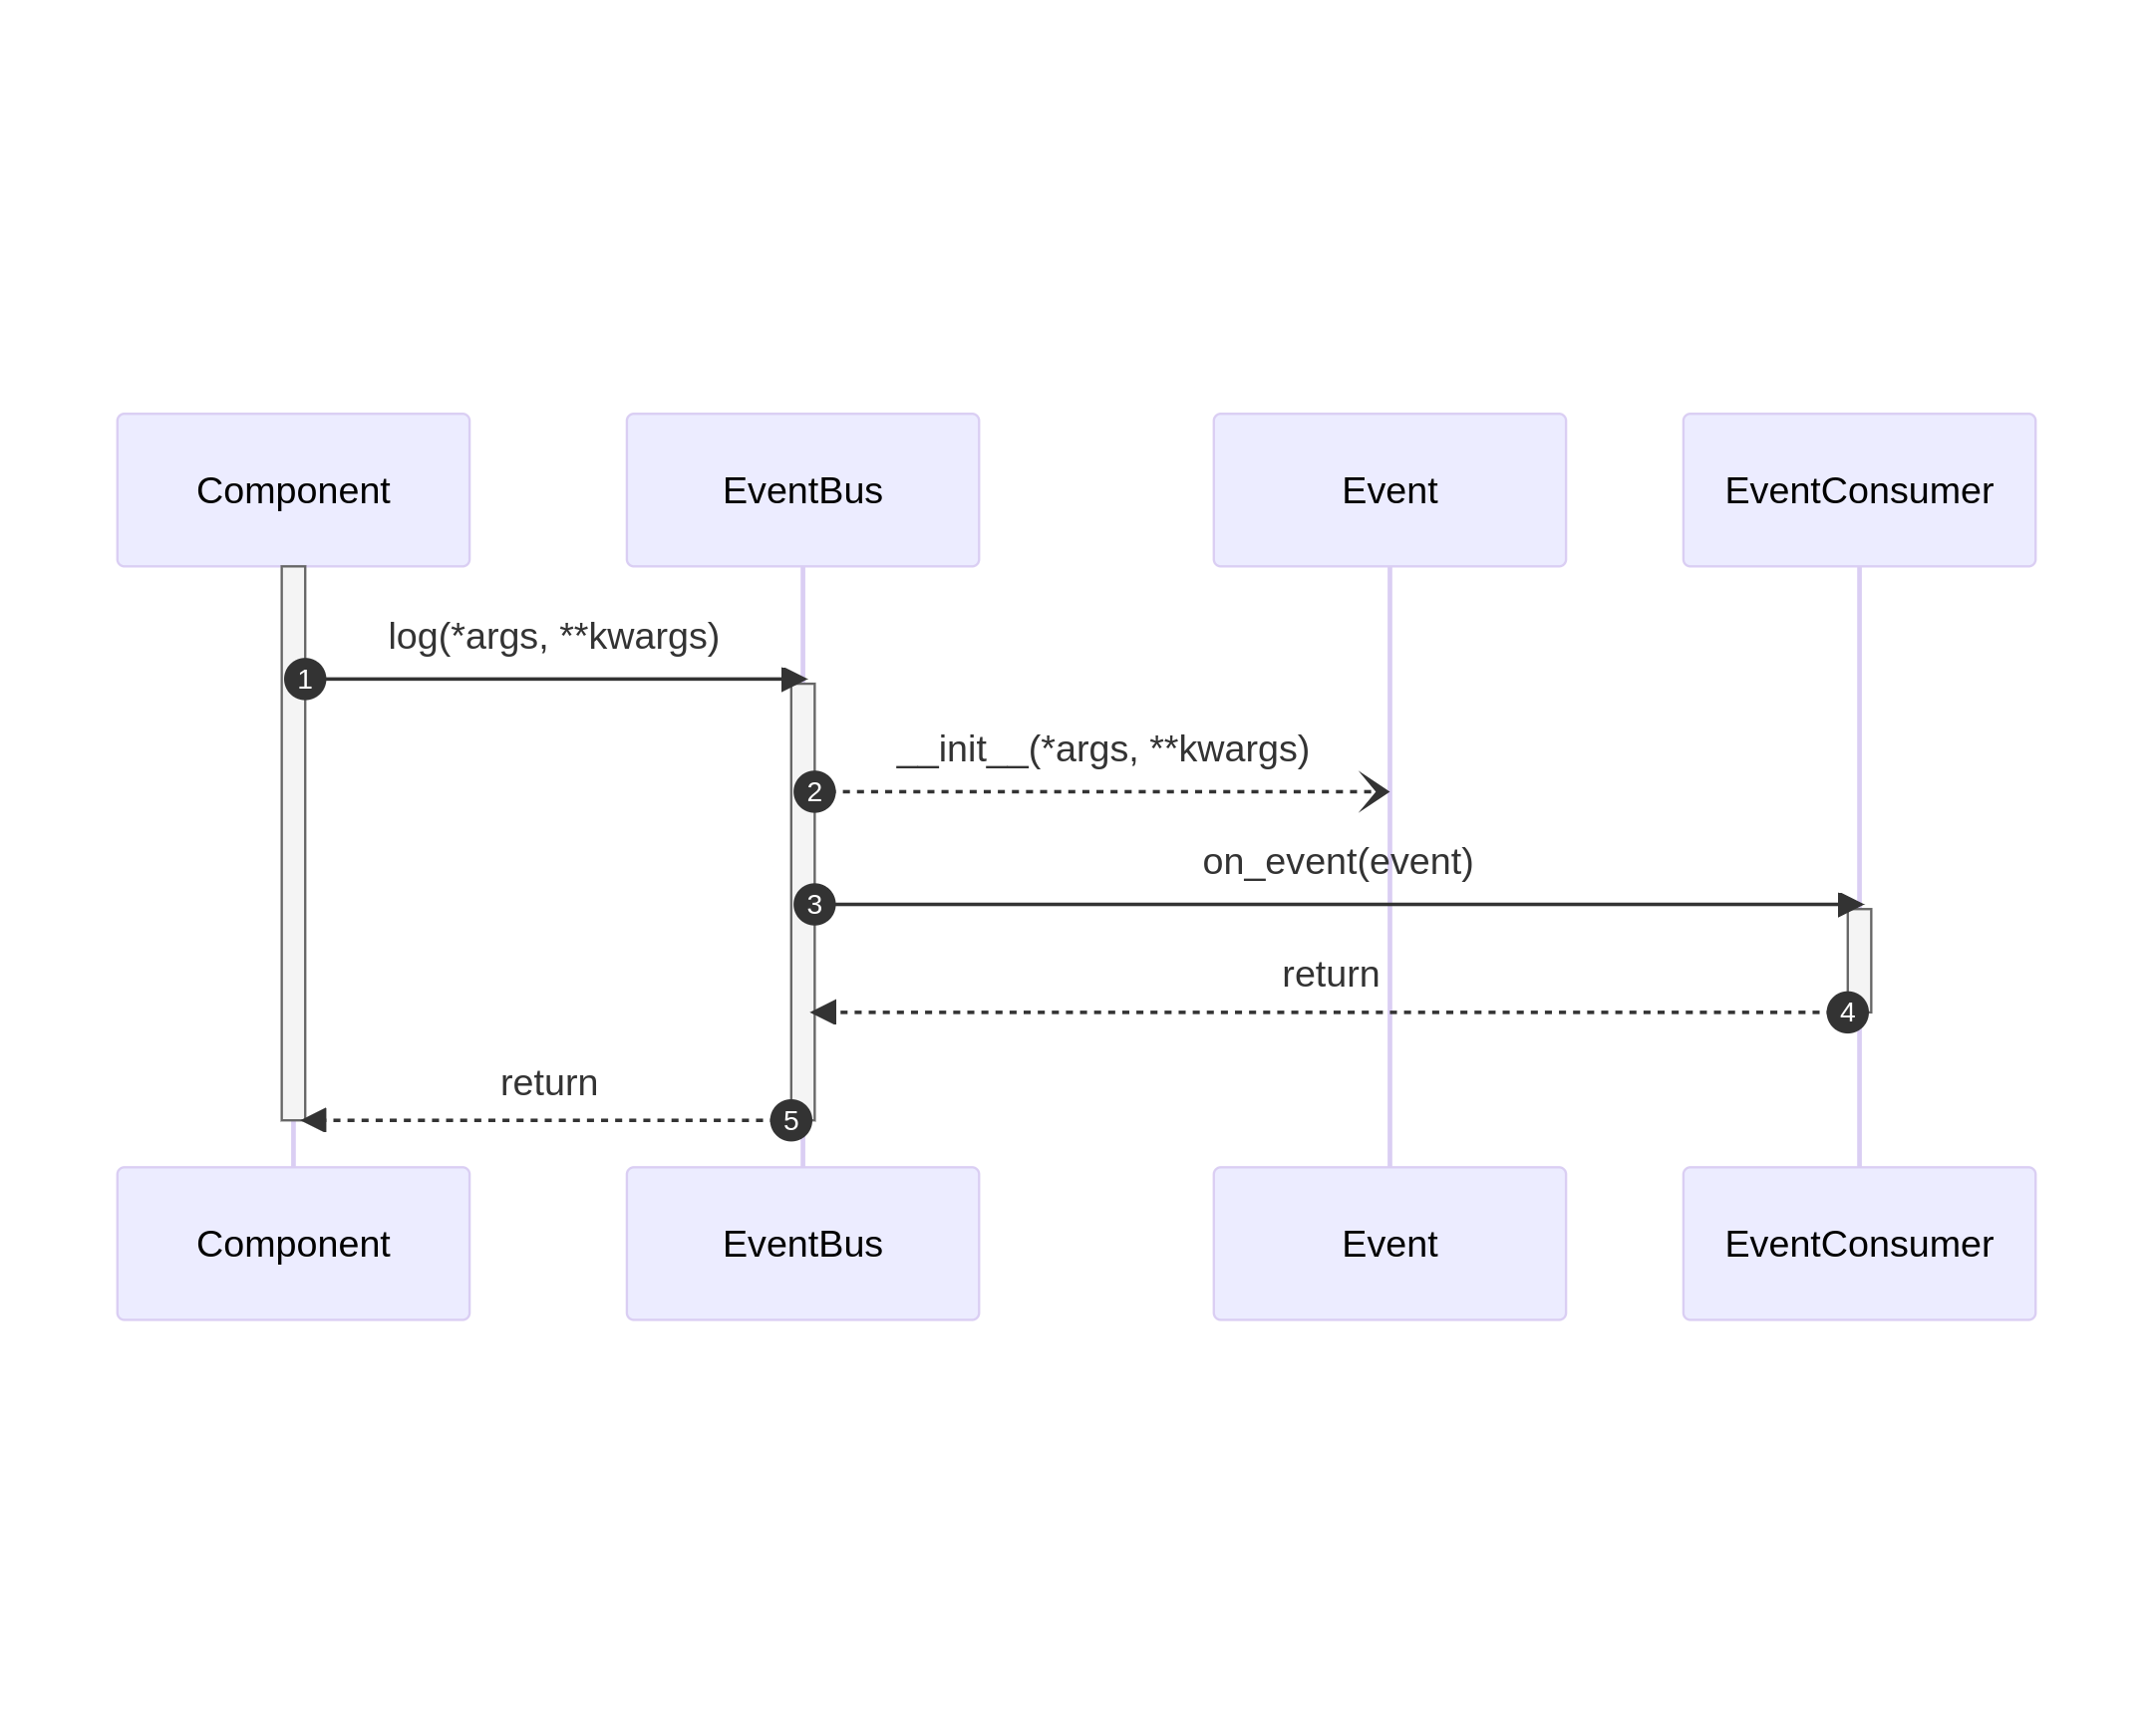
\includegraphics[width=0.75\linewidth]{images/diagrams/eventbus-v2-seq.png}
	\caption{Sequenzdiagramm Variante 2 Eventbus}
	\label{fig:eventbus-v2-seq}
\end{figure}
